The following demonstrates the calculation of output loss associated with the default using the growth accounting approach proposed by \citet{zarazaga-12}.

Following \citet{zarazaga-12}, assume that the production function follows the form $y_t = h^\alpha_t k^{1-\alpha}_t$ where $y_t$ denotes output, $k_t$ denotes physical capital, and $h_t$ denotes employment.
This implies that by the relationship $\frac{y_t}{h_t} = \left( \frac{k_t}{y_t} \right)^{\frac{1-\alpha}{\alpha}}$. If the capital-output ratio before the default episode $\kappa_b =\frac{k_b}{y_b}$ falls to $\kappa_a = \frac{k_{a}}{y_a}$ after the default episode, the output per worker would be
$\Delta = \left[\left(\frac{\kappa_a}{\kappa_b} \right)^{\frac{1-\alpha}{\alpha}} -1\right]\times 100$ percent higher.
If we ascribe all the observed decrease in capital to the sovereign default, we conclude that the output loss is on average $\frac{\Delta}{2} \%$ per worker during the period.
Note that $\left(\frac{\kappa_a}{\kappa_b} \right)^{\frac{1-\alpha}{\alpha}} -1 > 0$ if and only if $\kappa_a > \kappa_b$. This implies that there is an output loss only if the capital-output-ratio decreases. As argued in \citet{zarazaga-12}, the output loss is associated with a trough in the capital-output-ratio.

Using data from the Penn World Table, the annually capital-output ratio is calculated by dividing the capital stock at current PPPs (variable \emph{cn}) by the output-side real GDP at current PPPs (variable \emph{cgdpo}), both in million 2017 U.S. dollar.

In the case of Sri Lanka, capital-output ratio associated with the three default episodes (2005, 2012, 2017) recorded in the BoC-BoE Sovereign Default Database all increase, even for the consecutive years, as shown in Figure \ref{fig: sri-lanka-ky}. It is therefore unreasonable to attribute all the variations of the output to the sovereign default episodes.

For the case of Pakistan's biggest default in 1999, according to previous calibration, $\alpha=$ 0.4, which implies that by the relationship $\frac{y_t}{h_t} = \left( \frac{k_t}{y_t} \right)^{\frac{3}{2}}$.
Pakistan gained partial reaccess (debt flow > 0) and emerged from financial autarky in 2004 \citep{trebesch-2011-sovereign}, therefore the growth accounting will be conducted within 1999 to 2004.
The capital-output-ratio was about 1.36 in 1999. It rose to about 1.43 in 2003, and slowly fell to 1.4 in 2004, as shown in Figure \ref{fig: pakistan-ky}.
Following the exact same logic, since $\frac{k_t}{y_t}$ rose from 1.36 to 1.4 between 1999 and 2004, the output per worker actually increased, which is contradicting our assumption of an output loss.
Alternatively, if we consider the year of full reaccess as the end of default (debt flow > 1\% GDP), which is in 2006 \citep{trebesch-2011-sovereign}, the calculation yields that the output per worker would have been $ \left[\left(\frac{1.36}{1.355} \right)^{\frac{3}{2}} -1\right]\times 100 = $ 0.5\% higher, which gives an average output loss of 0.25\%. The value is too low compared to the average output loss of 5.5\% according to cross-country studies \citep{Uribe-Schmitt-Grohe-textbook,Borensztein-Panizza-defualt-cost}, which indicates that it is also unreasonable to ascribe all the effect on output to capital.
Hence, we conclude that the estimation of output cost of the default for Pakistan following \citet{zarazaga-12} is also not applicable.


\begin{figure}[t]
    \centering
    \begin{subfigure}[position]{0.49\textwidth}
        \centering
        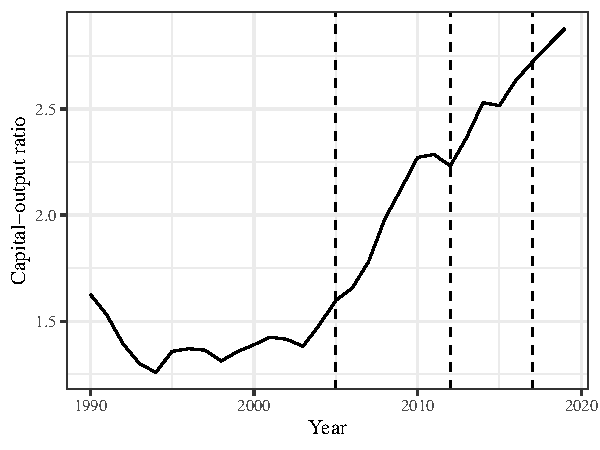
\includegraphics[width=\textwidth]{fig/sri_lanka_output_loss.pdf}
        \caption{Sri Lanka}
        \label{fig: sri-lanka-ky}
    \end{subfigure}
    \begin{subfigure}[position]{0.49\textwidth}
        \centering
        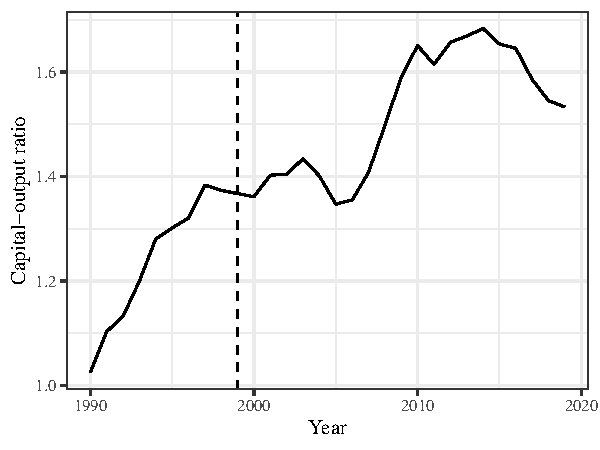
\includegraphics[width = \textwidth]{fig/pakistan_output_loss.pdf}
        \caption{Pakistan}
        \label{fig: pakistan-ky}
    \end{subfigure}
    \caption{Capital-Output Ratio, 1990 to 2020}
    \label{fig: LAK-PAK-ky}
    \floatfoot{Source: Penn World Table\\
    Note: The solid line represents the capital-output ratio for Sri Lanka and Pakistan. Default episode examined is plotted in vertical dashed lines.}
\end{figure}